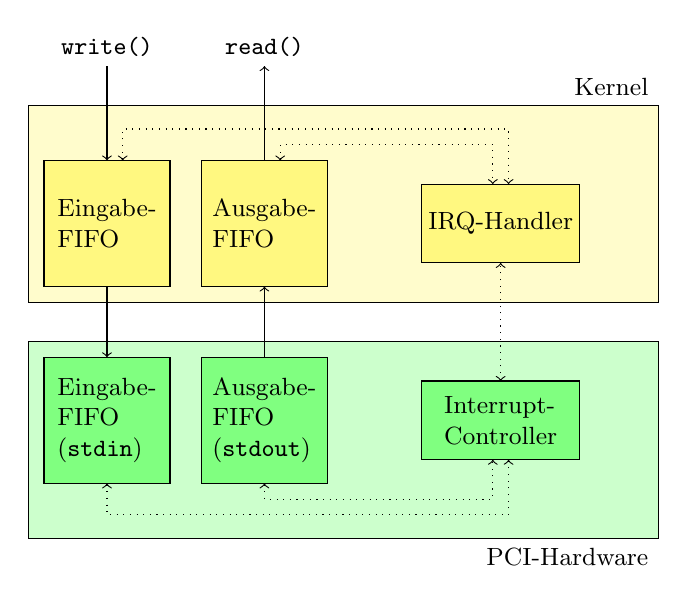
\begin{tikzpicture}
    \tikzstyle{every node}=[font=\small]
	\usetikzlibrary{positioning}
	\tikzstyle{pci}=[draw,fill=green!50,rectangle]
	\tikzstyle{krn}=[draw,fill=yellow!50,rectangle]
				
	\draw [fill=green!20] (0,-0.5) rectangle +(8,2.5);
	\draw [fill=yellow!20] (0,2.5) rectangle +(8,2.5);
				
	%\draw [<->] (1.8,0.9) -- (5,0.9);
	%\draw [<->] (3.8,1.1) -- (5,1.1);
	\draw [<->,dotted] (6,1.5) -- (6,3);
			
	\draw [<->,dotted] (1,0.2) -- (1,-0.2) -- (6.1,-0.2) -- (6.1,0.5);
	\draw [<->,dotted] (3,0.2) -- (3,-0) -- (5.9,0) -- (5.9,0.5);
				
	\draw [<->,dotted] (3.2,4.3) -- (3.2,4.5) -- (5.9,4.5) -- (5.9,4);
	\draw [<->,dotted] (1.2,4.3) -- (1.2,4.7) -- (6.1,4.7) -- (6.1,4);
				
	%\draw [<->] (1.8,3.4) -- (5,3.4);
	%\draw [<->] (3.8,3.6) -- (5,3.6);
				
	\node [anchor=north east] at (8,-0.5) {PCI-Hardware};
	\node [anchor=south east] at (8, 5.0) {Kernel};
				
	\draw [pci] (0.2,0.2) rectangle +(1.6,1.6) node [align=left,midway] {Eingabe-\\FIFO\\(\texttt{stdin})};
	\draw [pci] (2.2,0.2) rectangle +(1.6,1.6) node [midway,align=left] {Ausgabe-\\FIFO\\(\texttt{stdout})};
					
	\draw [krn] (0.2,2.7) rectangle +(1.6,1.6) node [midway,align=left] {Eingabe-\\FIFO};
	\draw [krn] (2.2,2.7) rectangle +(1.6,1.6) node [midway,align=left] {Ausgabe-\\FIFO};
				
	\draw [->] (1,2.7) -- (1,1.8);
	\draw [<-] (3,2.7) -- (3,1.8);
				
	\draw [->] (1,5.5) -- (1,4.3);
	\draw [<-] (3,5.5) -- (3,4.3);
	\node [anchor=south] at (3,5.5) {\texttt{read()}};
	\node [anchor=south] at (1,5.5) {\texttt{write()}};
				
	\draw [pci] (5,0.5) rectangle +(2,1) node [align=left,midway] {Interrupt-\\Controller};
		\draw [krn] (5,3) rectangle +(2,1) node [midway] {IRQ-Handler};
\end{tikzpicture}